\documentclass[11pt]{article}
\usepackage{acl2016}
\usepackage[utf8]{inputenc}
\usepackage{times}
\usepackage{latexsym}
\usepackage{graphicx}
\usepackage{multirow}

\aclfinalcopy 
%\def\aclpaperid{***}

\newcommand\BibTeX{B{\sc ib}\TeX}
\newcommand*\rot{\rotatebox{90}}

\title{Automatic Classification by Topic Domain for Meta Data Generation, Web Corpus Evaluation, and Corpus Comparison}

\author{Roland Schäfer\\
	    Freie Universität Berlin\\
	    Habelschwerdter Allee 45\\
	    14196 Berlin, Germany\\
	    {\tt roland.schaefer@fu-berlin.de}
	  \And
	Felix Bildhauer\\
  	Institut für Deutsche Sprache\\
  	R5, 6--13\\
  	68161 Mannheim, Germany\\
  {\tt bildhauer@ids-mannheim.de}}

\date{}

\begin{document}

\maketitle

\begin{abstract}
In this paper, we describe preliminary results from an ongoing experiment wherein we classify two large unstructured text corpora---a web corpus and a
newspaper corpus---by topic domain (or subject area).
Our primary goal is to develop a method that allows for the reliable annotation of large crawled web corpora with meta data required by many corpus linguists. We are especially interested in designing an annotation scheme whose categories are both intuitively interpretable by linguists and firmly rooted in the distribution of lexical material in the documents.
Since we use data from a web corpus and a more traditional corpus, we also contribute to the important field of corpus comparison and corpus evaluation.
Technically, we use (unsupervised) topic modeling to automatically induce topic distributions over gold standard corpora that were manually annotated for 13 coarse-grained topic domains.
In a second step, we apply supervised machine learning to learn the manually annotated topic domains using the previously induced topics as features.
We achieve around 70\% accuracy in 10-fold cross validations.
An analysis of the errors clearly indicates, however, that a revised classification scheme and larger gold standard corpora will likely lead to a substantial increase in accuracy.
\end{abstract}

\section{Introduction}
\label{sec:introduction}

In the experiment reported here, we classified large unstructured text corpora by \textit{topic domain}.
The \textit{topic domain} of a document---along with other high-level classifications such as \textit{genre} or \textit{register}---is among the types of meta data most essential to many corpus linguists.
Therefore, the lack of reliable meta data in general is often mentioned as a major drawback of large, crawled web corpora, and the automatic generation of such meta data is an active field of research.\footnote{See, for example, many of the contributions in \newcite{MehlerEa2010}.}
It must be noted, however, that such high-level annotations are not reliably available for many very large traditional corpora (such as newspaper corpora), either.
When it comes to the automatic identification of high-level categories like register (such as \textit{Opinion}, \textit{Narrative}, \textit{Informational Persuation}; Biber and Egbert 2016), even very recent approaches based on very large amounts of training data cannot deliver satisfying (arguably not even encouraging) results.
For instance, \newcite[23]{BiberEgbert2016} report \textit{accuracy}=$0.421$, \textit{precision}=$0.268$, \textit{recall}=$0.3$.
It is not even clear whether categories such as register and genre can be operationalized such that a reliable annotation is possible for humans.

By contrast, automatic text categorization by \textit{content} yielded much more promising results years ago already \cite{Sebastiani2002}.
Furthermore, data-driven induction of topics (\textit{topic modeling}) has proven quite successful, and it is in many respects a very objective way of organizing a collection of documents by content.
Deriving topic classifications from text-internal criteria is also advocated in the \newcite{EAGLES1996} guidelines, among others.
However, topic modeling usually does not come with category labels that are useful for linguistic corpus users.
In our project, we explore the possibility of inferring a small, more traditional set of \textit{topic domains} (or \textit{subject areas}) from the topics induced in an unsupervised manner by Latent Semantic Indexing \cite{LandauerDumais1994,LandauerDumais1997}.
Since we classify and compare one large German web corpus and one large German newspaper corpus with respect to their distribution of topic domains, our paper also contributes to the area of corpus comparison, another important issue in corpus linguistics \cite{Kilgarriff2001,BiemannEa2013}.
For the construction of crawled web corpora, such comparisons are vital because next to nothing is known about their composition.

The computational tools used in our method (unsupervised topic induction and supervised classifiers) are by now well-established and highly developed.
This paper contributes to the field of applying such methods and making them usable for real-life problems of data processing and the development of suitable annotation schemes rather than to the development of the underlying mathematics and algorithms.

\section{Gold Standard Data}
\label{sec:goldstandard}

Our gold standard corpora were prepared by manual annotation of documents from two large German corpora.
The first data set consists of 870 randomly selected documents from DECOW14A, a crawled web corpus \cite{SchaeferBildhauer2012a,Schaefer2015b}, henceforth \textit{Web}.
The second data set contains 886 documents randomly selected from DeReKo, a corpus composed predominantly of newspaper texts \cite{KupietzEa2010}, henceforth \textit{News}. 
Our choice of corpora was motivated by fact that we expected some overlap w.\,r.\,t.\ to topics covered in them, but also some major differences. 
The documents in these gold standard corpora were classified according to a custom annotation scheme for topic domain which builds on previous work by \newcite{Sharoff2006}.
The design goal was to a have moderate number (about 10--20) of topic domains that can be thought of as subsuming more fine-grained topic distinctions.
We developed the annotation scheme in a cyclic fashion, taking into account annotator feedback after repeated annotation processes.
For the experiment reported here, we used a version that distinguishes 13 topic domains, namely \textit{Science}, \textit{Technology}, \textit{Medical}, \textit{Public Life and Infrastructure}, \textit{Politics and Society}, \textit{History}, \textit{Business}, \textit{Law}, \textit{Fine Arts},  \textit{Philosophy}, \textit{Beliefs},  \textit{Life and Leisure}, \textit{Individuals}.

\begin{figure*}[!ht]
  \centering
  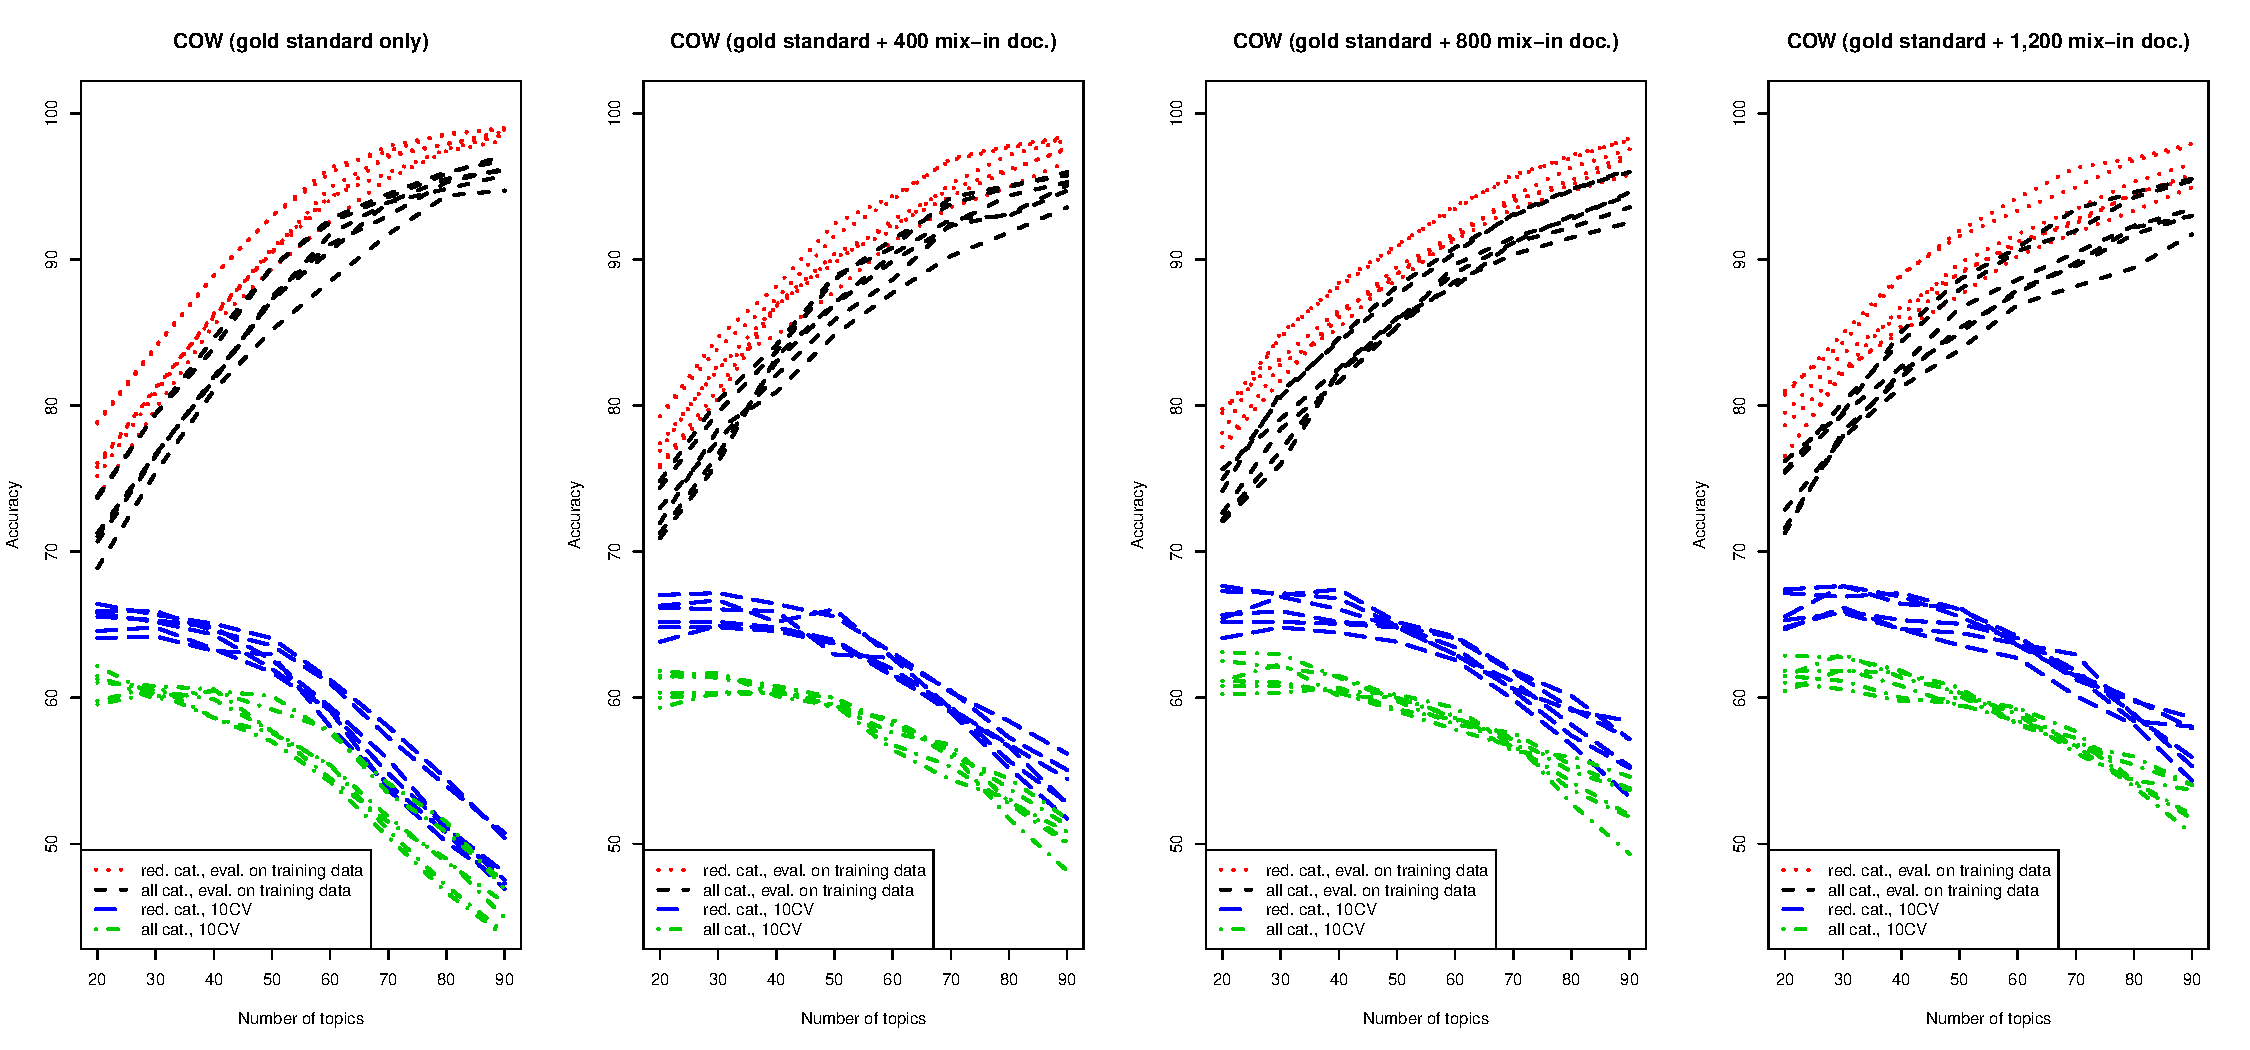
\includegraphics[width=\textwidth, height=6.4cm]{graphics/cow.pdf}
  \caption{Accuracy with different numbers of topics for the Web dataset}
  \label{fig:cow}
\end{figure*}

\section{Experiment Setup}
\label{sec:experiment}

Our general approach was to infer a topic distribution over a corpus using \textit{unsupervised} topic modeling algorithms as a first step.
In the second step, rather than examining and interpreting the inferred topical structure, we used the resulting document--topic matrix to learn topic domain distinctions for the documents from their assignment to the topics in a \textit{supervised} manner.
To achieve this, supervised classifiers were used.
Through permutation of virtually all available classifiers (with the appropriate capabilities) available in the Weka toolkit \cite{HallWitten2011}, LM Trees \cite{LandwehrEa2005} and SVMs with a Pearson VII kernel \cite{UstunEa2006} were found to be most accurate.
Due to minimally higher accuracy, SVMs were used in all subsequent experiments.
Some topic domains occurred only rarely in the gold standard, and we did not expect the classifier to be able to generalize well from just a few instances.
Therefore, we evaluated the results on the \textit{full} data set and a \textit{reduced} data set with rare categories removed.

For the first step (unsupervised topic induction), we used LSI and LDA (Latent Dirichlet Allocation, Blei et al.\ 2003\nocite{BleiEa2003}) as implemented in the Gensim toolkit \cite{RehurekSojka2010}.
In our first experiments, the LDA topic distribution was unstable, and results were generally unusable, possibly due to the comparatively small gold standard corpora used.
We consequently only report LSI results here and will return to LDA in further experiments (cf. Section~\ref{sec:conclusions}).
However, for any topic modeling algorithm, our corpora can be considered small.
Therefore, we inferred topics not just based on the annotated gold standard data sets, but also on larger datasets which consisted of the gold standard mixed with additional documents from the source corpora.
For the training of the SVM classifiers, the documents that had been mixed in were removed again because no gold standard annotation was available for them.
We systematically increased the number of mixed-in document in increments of roughly half as many documents as contained in the gold standard corpora.

We pre-processed both corpora in exactly the same way (tokenization, lemmatization, POS-tagging, named entity recognition).
Using the lemma and the simplified POS tags (such as \textit{kindergarten\_nn}) as terms in combination with some filters (use only lower-cased purely alphabetic common and proper noun lemmas between 4 and 30 characters long) usually gave the best results.

\section{Results}
\label{sec:results}

\begin{figure*}[!ht]
  \centering
  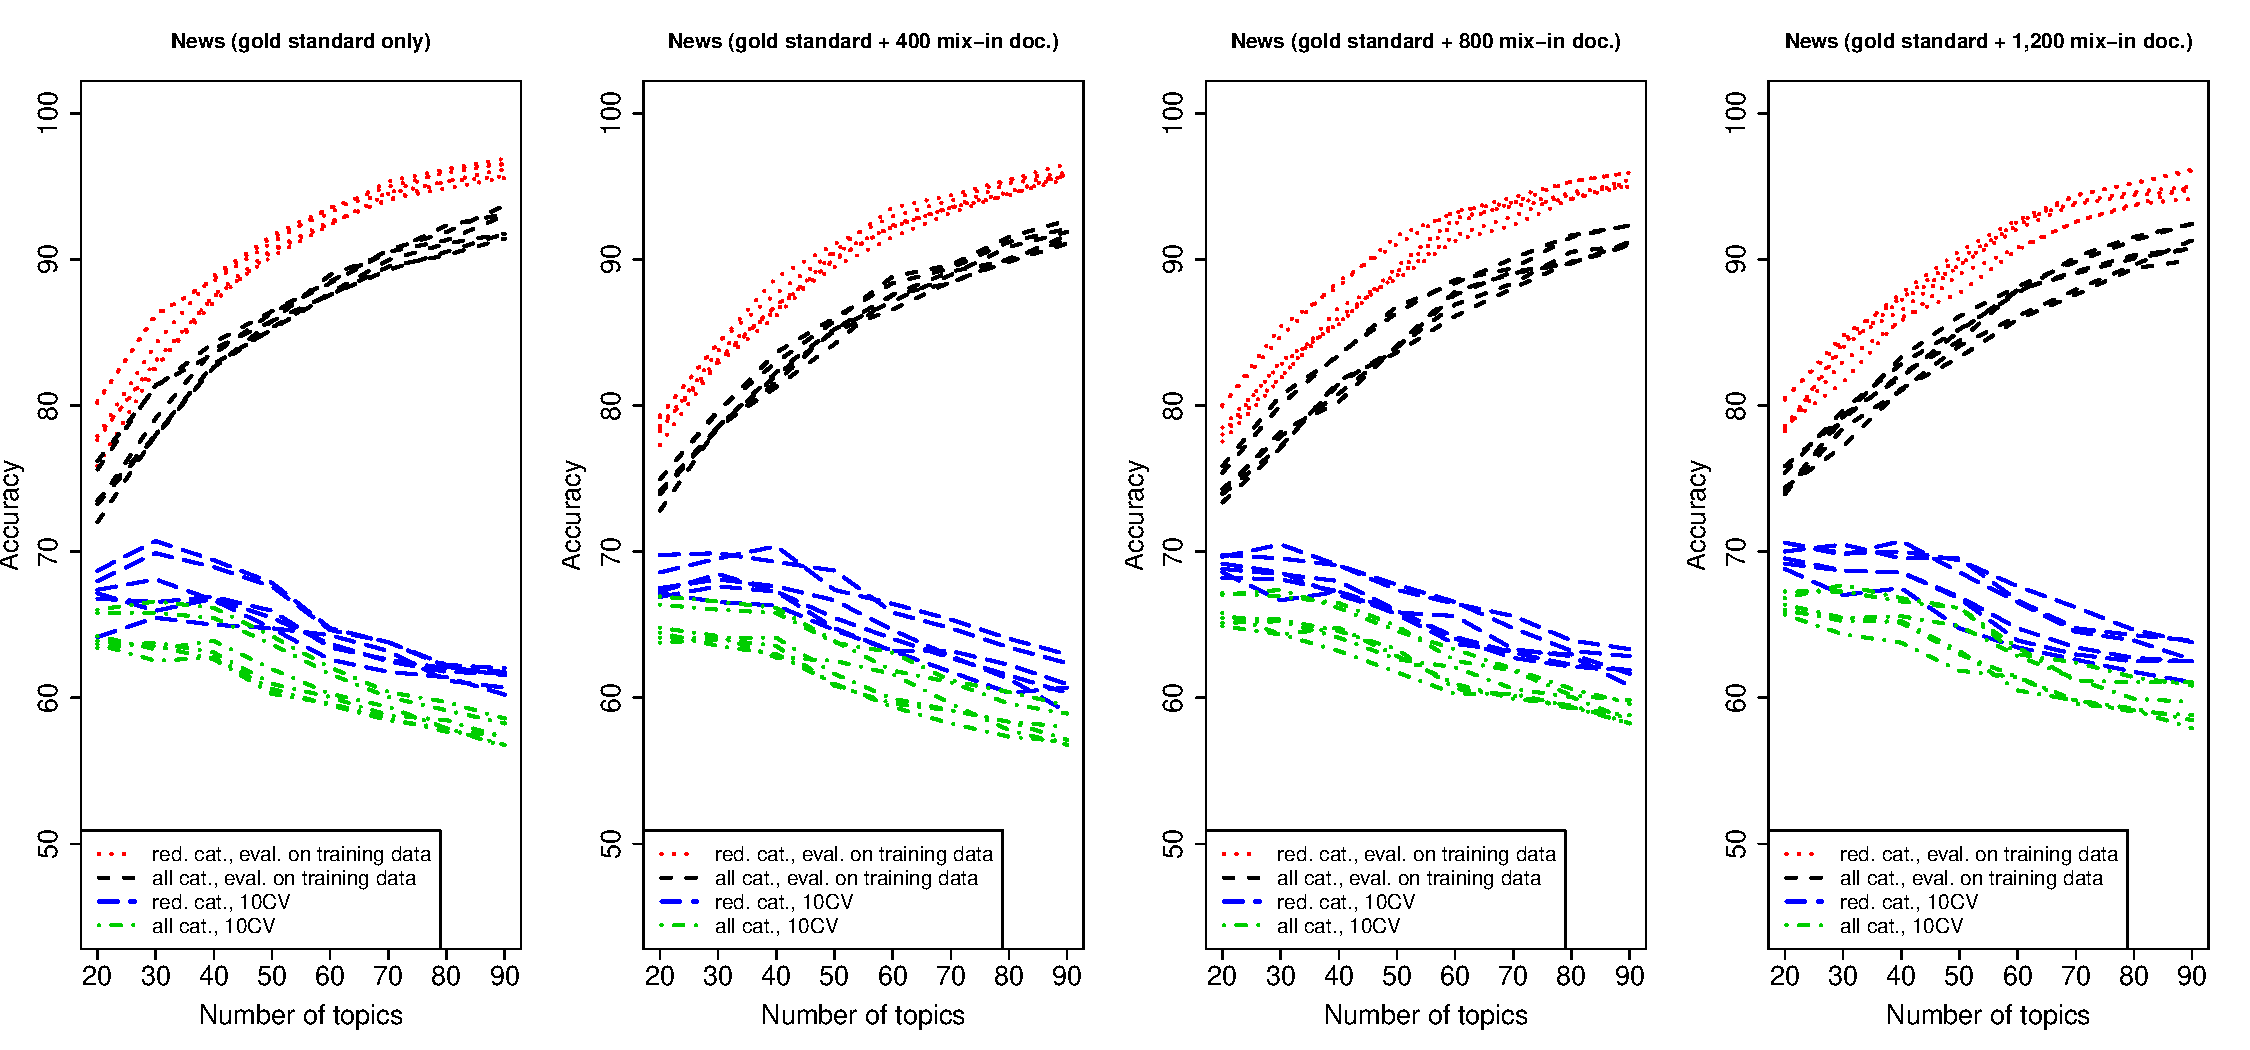
\includegraphics[width=\textwidth, height=6.4cm]{graphics/dereko.pdf}
  \caption{Accuracy with different numbers of topics for the News dataset}
  \label{fig:dereko}
\end{figure*}

\begin{table*}[!ht]
  \centering
  \resizebox{\textwidth}{!}{\begin{tabular}{|lrllrrrr|}
    \hline
    \textbf{Corpus} & \textbf{Mixed-in} & \textbf{Attribute} & \textbf{Topics} & \textbf{Accuracy} & \textbf{Precision}$^{\mathrm{\tiny *}}$ & \textbf{Recall}$^{\mathrm{\tiny *}}$ & \textbf{F-Measure}$^{\mathrm{\tiny *}}$ \\
    \hline
    Web & 3,200 & token & 20 & 68.765\% & 0.688 & 0.688 & 0.674 \\
    News & 3,600 & lemma + POS & 40 & 72.999\% & 0.725 & 0.730 & 0.696 \\
    Web + News & 0 & lemma + POS & 30 & 51.872\% & 0.431 & 0.519 & 0.417 \\ 
    \hline
  \end{tabular}}
  \caption{Evaluation at best achievable accuracy with the reduced set of topic domains in 10-fold cross-validation ($^{\mathrm{\tiny *}}$weighted average across all categories)}
  \label{tab:quality}
\end{table*}

Figure~\ref{fig:cow} shows the classification accuracy using 20 to 90 LSI topics.
Each line corresponds to one sub-experiment (with slightly different pre-processing options for lines of the same color and style), and the lines form well distinguishable bands.
The highest accuracy is achieved with the reduced set of topic domains (minor categories removed) when the evaluation is performed on the training data.
The full set of topic domains leads to a drop in accuracy of about 5\%.
The two lower bands show the classification accuracy in a 10-fold cross-validation (10CV), again with the reduced set of topic domains performing roughly 5\% better.
While a higher number of topics improves results on the training data, the accuracy in the cross-validation drops.
Too large numbers of topics obviously allow the method to pick up idiosyncratic features of single documents or very small clusters of documents, leading to extreme overfitting.

The four panels show results based on different topic models.
Panel (a) uses a topic model inferred only from the (more than 800) gold standard documents.
Results in panel (b) through (d) are based on topic models inferred on larger data sets as described in Section~\ref{sec:experiment}.
In the experiment reported in panel (d), for example, 1,200 documents were added to the 870 gold standard documents.
While the results of the 10CV are slightly improved by mixing in more documents, the maximum achieved accuracy does not change significantly.
We mixed in up to 8,000 additional documents (not all results shown here) with no significant change compared to panel (d) in Figure~\ref{fig:cow}.
We consider the maximum 10CV accuracy with the reduced set of topic domains most informative w.\,r.\,t.\ the potential quality of our method, and we report it in Table~\ref{tab:quality}.

\begin{figure*}[!ht]
  \centering
  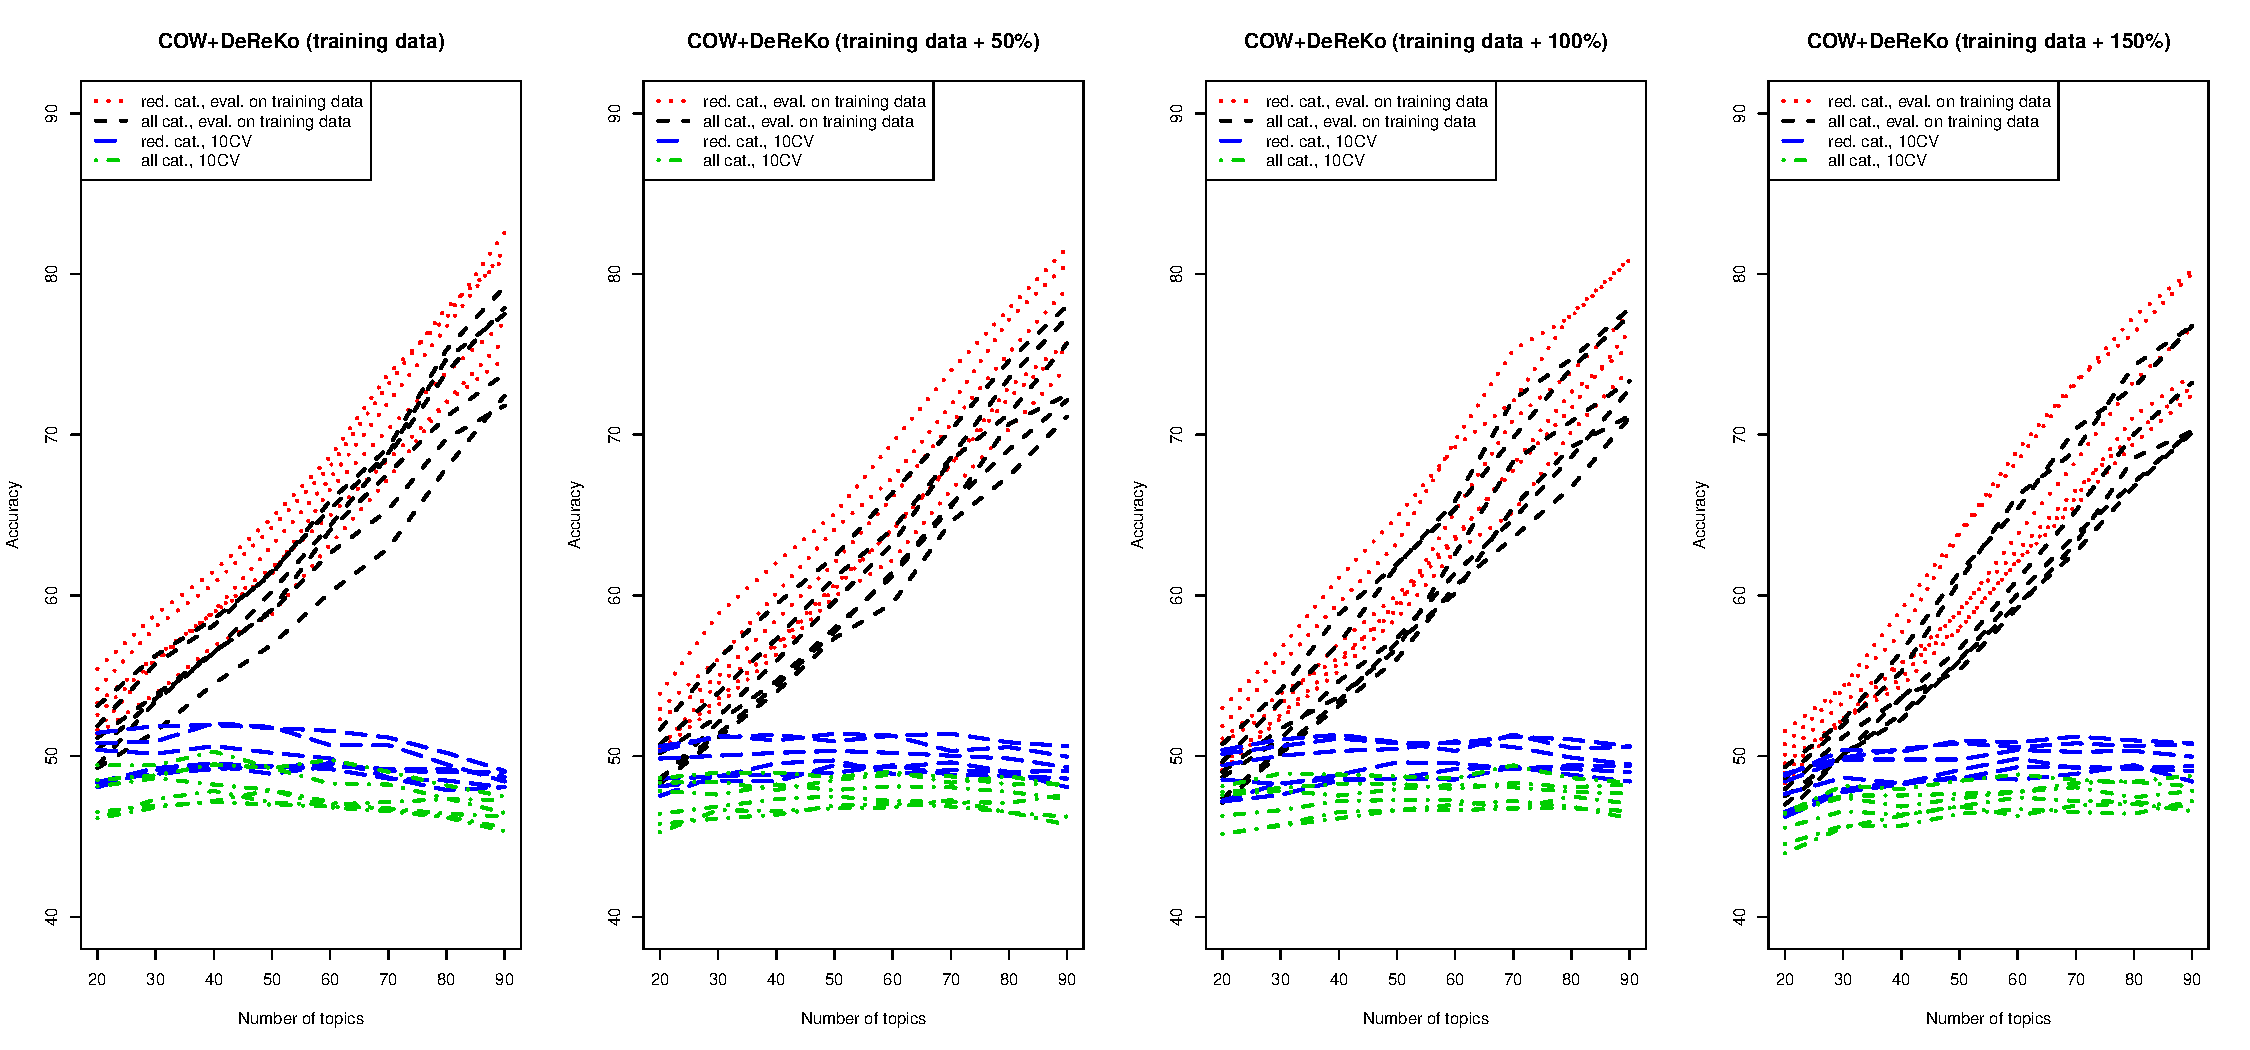
\includegraphics[width=\textwidth, height=6.4cm]{graphics/coreko.pdf}
  \caption{Accuracy with different numbers of topics for the pooled Web + News datasets}
  \label{fig:coreko}
\end{figure*}

A very similar plot for the News data is shown in Figure~\ref{fig:coreko}.
The best results are also given in Table~\ref{tab:quality}.
The added accuracy (4.23\% according to Table~\ref{tab:quality}) is a side effect of the more skewed distribution of topic domains in the News gold standard data.

The $\kappa$ statistic for the Web and Newspaper results from Table~\ref{tab:quality} is $\kappa_{\textrm{\tiny Web}}=0.575$ and $\kappa_{\textrm{\tiny News}}=0.582$, indicating that achieving a higher accuracy for the web data is actually slightly harder than for the newspaper data (see also the analysis of the confusion matrices below).

\enlargethispage{\baselineskip}
When the Web and News data are pooled, however, quality drops below any acceptable level, cf.\ Figure~\ref{fig:coreko} and Table~\ref{tab:quality}.
Mixing in more documents (panels b--d) improves the evaluation results on the training data, but the 10CV results remains steady at around 50\%.
This is remarkable because larger training data sets should lead to increased, not degraded accuracy.
While a deeper analysis of the LSI topic distributions remains to be undertaken, it is evident what most likely causes these below average results on the side of the SVM classifier when looking at the confusion matrices, cf.\ Table~\ref{tab:confusion}.
In the Web gold standard (panel a), the dominant modal category is \textit{Life and Leisure}.
The distribution of topic domains is reasonably skewed, and the confusion is distributed roughly uniformly across categories.
The News gold standard (panel b) consists mainly of two clusters of documents in the domains \textit{Politics and Society} and \textit{Life and Leisure}.
For the pooled data set (panel c), this leads to a situation in which the classifier simply assigns most documents to \textit{Life and Leisure} and the rest mostly to \textit{Politics and Society}.
This indicates that for such skewed distributions of topic domains, larger gold standard data sets are required.
It is not indicative of a general failure of the method or a general incompatibility of newspaper and web data in the context of our method.
The confusion matrices in Table~\ref{tab:confusion} clearly indicate, however, that topic domains are represented quite differently in newspaper and web corpora.

\begin{table*}[!ht]
  \centering
  \resizebox{0.33\textwidth}{!}{\begin{tabular}{|llcccccccc|}
    \hline
    \multicolumn{2}{|c}{\textbf{Web}} & \multicolumn{8}{c|}{\textbf{Classified}} \\
     && \rot{\textbf{PolSoc~}} & \rot{\textbf{Busi}} & \rot{\textbf{Life}} & \rot{\textbf{Arts}} & \rot{\textbf{Public~}} & \rot{\textbf{Law}} & \rot{\textbf{Beliefs~}} & \rot{\textbf{Hist}} \\
   \hline
   \multirow{8}{*}{\rot{\textbf{Annotated}}} & \textbf{PolSoc}  & \textbf{26} &  12 &  10 &   1 &   1 &   0 &   1 &   0 \\ 
     & \textbf{Busi}    &  5 & \textbf{105} &  40 &   7 &   1 &   2 &   1 &   1 \\ 
     & \textbf{Life}    &  3 &  14 & \textbf{286} &   6 &   4 &   1 &   1 &   1 \\ 
     & \textbf{Arts}    &  3 &   2 &  36 &  \textbf{78} &   1 &   0 &   2 &   6 \\ 
     & \textbf{Public}  &  0 &   3 &  11 &   0 &   \textbf{9} &   1 &   0 &   0 \\ 
     & \textbf{Law}     &  3 &   9 &   8 &   0 &   1 &   \textbf{8} &   0 &   0 \\ 
     & \textbf{Beliefs} &  4 &   3 &  11 &   6 &   1 &   0 &  \textbf{30} &   1 \\ 
     & \textbf{Hist}    &  9 &   0 &   9 &   7 &   1 &   1 &   2 &  \textbf{15} \\ 
     \hline
 \end{tabular}}~~\resizebox{0.323\textwidth}{!}{\begin{tabular}{|llcccccc|}
    \hline
     \multicolumn{2}{|c}{\textbf{News}} & \multicolumn{6}{c|}{\textbf{Classified}} \\
     && \rot{\textbf{PolSoc~}} & \rot{\textbf{Busi}} & \rot{\textbf{Life}} & \rot{\textbf{Indiv}} & \rot{\textbf{Arts}} & \rot{\textbf{Public}} \\
    \hline
     \multirow{6}{*}{\rot{\textbf{Annotated}}}& \textbf{PolSoc}  & 223 & 6 & 39 &  0 &  0 &  8 \\
     & \textbf{Busi}    &  20 & 24 &   9 &  0 &  0 &  0 \\
     & \textbf{Life}    &  24 &  1 & 324 &  0 &  0 &  1 \\
     & \textbf{Indiv}   &   5 &  0 &  17 &  0 &  0 &  1 \\
     & \textbf{Arts}    &   2 &  0 &  28 &  0 &  6 &  0 \\
     & \textbf{Public}  &  35 &  0 &  30 &  0 &  0 & 34 \\
    \hline
 \end{tabular}}~~\resizebox{0.315\textwidth}{!}{\begin{tabular}{|llccccccccc|}
    \hline
     \multicolumn{2}{|c}{\textbf{Pooled}} & \multicolumn{9}{c|}{\textbf{Classified}} \\
     && \rot{\textbf{PolSoc~}} & \rot{\textbf{Busi}} & \rot{\textbf{Medical~}} & \rot{\textbf{Life}} & \rot{\textbf{Arts}} & \rot{\textbf{Public~}} & \rot{\textbf{Law}} & \rot{\textbf{Beliefs~}} & \rot{\textbf{Hist}} \\
    \hline
    \multirow{9}{*}{\rot{\textbf{Annotated}}} & \textbf{PolSoc}   & \textbf{199} &   7 &   0 & 109 &   0 &  12 &   0 &   0 &   0 \\ 
    & \textbf{Busi}     &  18 &  \textbf{23} &   0 & 172 &   0 &   2 &   0 &   0 &   0 \\ 
    & \textbf{Medical}  &   6 &   0 &   \textbf{0} &  29 &   0 &   1 &   0 &   0 &   0 \\ 
    & \textbf{Life}     &  25 &   4 &   0 & \textbf{632} &   0 &   5 &   0 &   0 &   0 \\ 
    & \textbf{Arts}     &   2 &   2 &   0 & 160 &   \textbf{0} &   0 &   0 &   0 &   0 \\ 
    & \textbf{Public}   &  46 &   2 &   0 &  56 &   0 &  \textbf{19} &   0 &   0 &   0 \\ 
    & \textbf{Law}      &   8 &   0 &   0 &  31 &   0 &   0 &   \textbf{0} &   0 &   0 \\ 
    & \textbf{Beliefs}  &   0 &   0 &   0 &  59 &   0 &   0 &   0 &   \textbf{0} &   0 \\ 
    & \textbf{Hist}     &   4 &   0 &   0 &  50 &   0 &   0 &   0 &   0 &   \textbf{0} \\ 
    \hline
 \end{tabular}}
  \caption{Confusion matrices for the best achievable results on the Web (a), News (b), and pooled (c) data sets as reported in Table~\ref{tab:quality}; different sets of categories are the result of excluding low-frequency topic domains (below 20 for Web and News, below 30 for pooled data)}
  \label{tab:confusion}
\end{table*}

\section{Conclusions and Outlook}
\label{sec:conclusions}

The results presented here are highly encouraging, and they clearly indicate the route to be taken in further experiments.
First of all, there appears to be a connection between induced topic distributions and more general topic domains.
The decreased performance in cross-validation experiments indicates that larger gold standard data sets are required.
Such data sets are currently being annotated under our supervision.

\pagebreak

Secondly, there appears to be a significant difference in the topic distribution and the topic\slash domain mapping in newspaper and web corpora.
This might be one of the reasons behind the collapse of the classifier when newspaper and web data are pooled.
In future experiments, it remains to be discovered whether larger gold standard corpora can alleviate such problems.
This will eventually enable us to decide whether separate models or pooled models for the two kinds of corpora are more appropriate.

Thirdly, the highly skewed topic distributions in both newspaper and web corpora indicate that splitting up some topic domains might lead to a better fit.
In fact, annotators have independently asked whether \textit{Politics and Society} and \textit{Life and Leisure}---the critical categories which make the classifier collapse (cf.\ Section~\ref{sec:results})---could not be split up into at least two categories each.

Additionally, we will investigate whether alternative topic modeling algorithms lead to a better fit.%
\footnote{The Gensim toolkit offers a wide array of algorithms, including \textit{doc2vec} and an alternative LDA implementation \textit{ldamallet}.}
Moreover, as suggested by an anonymous reviewer, our results could be compared with a baseline classification that does not make use of topic modeling algorithms.
Finally, we are currently experimenting with an extended annotation scheme that allows for multiple weighted assignments of documents to topic domains.

The ultimate goal of our project is to automatically annotate existing web corpora that are several billion tokens large with meta data such as their topic domain and to release the data freely (under a maximally permissive Creative Commons Attribution license).%
\footnote{The software and the classifiers will be made available under permissive open source licenses allowing even their use in commercial applications.}
The experiments reported here indicate that with some tweaking, it will be possible to create such free resources and achieve very high levels of quality.

\section*{Acknowledgments}

Roland Schäfer's research on the project presented here was funded by the German Research Council (Deutsche Forschungsgemeinschaft, DFG) through grant SHA/1916-1 \textit{Linguistic Web Characterization}.

\bibliography{coreko}
\bibliographystyle{acl2016}

\end{document}
